% author_config.tex (gitignored)
\newcommand{\authorname}{Ryan Sherrington}
\newcommand{\authoremail}{ryan.sherrington@gmx.co.uk}
\documentclass[11pt]{article}
\usepackage{graphicx}
\usepackage{hyperref}
\title{Plasma Vortex Reactor: CI-validated Modeling with Stability KPI Gates and Dynamic Ripple Control}
\author{See author\_config.tex}
\date{\today}
\begin{document}
\maketitle
\begin{abstract}
We present a reproducible modeling and validation pipeline for a plasma vortex reactor with CI-enforced KPI gates, dynamic ripple control, and artifact-rich reporting.
\end{abstract}
\section{Introduction}
Motivation and contributions.
\section{Methods}
Outline of reactor model, dynamic ripple, and CI.
\section{Results}
\subsection{Operating Envelope} See Fig.~\ref{fig:envelope}.
\subsection{KPI Gates and Ripple} See Fig.~\ref{fig:ripple}.
\section{Reproducibility}
Bundle, schemas, and CI.
\section{Conclusion}
Future work.
\begin{figure}[h]
\centering
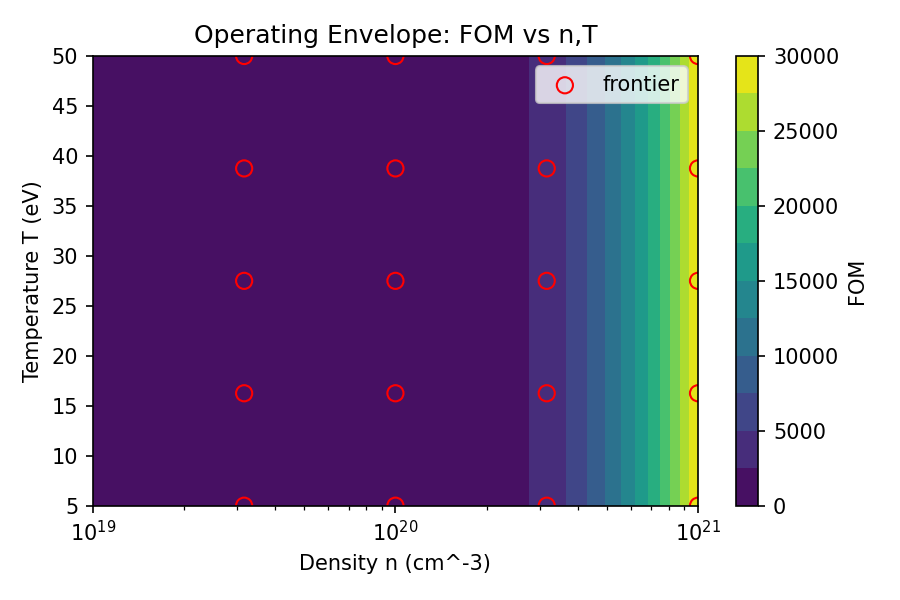
\includegraphics[width=0.7\linewidth]{operating_envelope.png}
\caption{Operating envelope (FOM vs n,T).}\label{fig:envelope}
\end{figure}
\begin{figure}[h]
\centering
\includegraphics[width=0.6\linewidth]{dynamic_stability_ripple.png}
\caption{Stability vs ripple with gate.}\label{fig:ripple}
\end{figure}
\end{document}
